\documentclass[a4paper,11pt]{article}
\input{/home/tof/Documents/Cozy/latex-include/preambule_lua.tex}
\newcommand{\showprof}{show them}  % comment this line if you don't want to see todo environment
\fancyhead[L]{Devinette du berger}
\newdate{madate}{10}{09}{2020}
%\fancyhead[R]{\displaydate{madate}} %\today
%\fancyhead[R]{Seconde - SNT}
%\fancyhead[R]{Première - NSI}
\fancyhead[R]{Terminale - NSI}
\fancyfoot[L]{~\\Christophe Viroulaud}
\AtEndDocument{\label{lastpage}}
\fancyfoot[C]{\textbf{Page \thepage/\pageref{lastpage}}}
\fancyfoot[R]{\includegraphics[width=2cm,align=t]{/home/tof/Documents/Cozy/latex-include/cc.png}}
\usepackage{tikz}
\usetikzlibrary{shapes.multipart}
\begin{document}
\begin{Form}
\section{Présentation}
Une devinette raconte l’histoire d’un berger qui possède un chou, une chèvre et un loup. En sa présence, la chèvre n’ose pas manger le chou, pas plus que le loup n’ose manger la chèvre, mais ils n’hésiteraient pas à satisfaire leurs appétits si l’homme tournait le dos. Ce berger doit traverser une rivière avec sa petite troupe et il ne dispose que d’une barque, dans laquelle il peut naviguer avec un seul de ses compagnons.
\begin{center}
\shadowbox{\parbox{10cm}{\centering Peut-on résoudre cette devinette par un graphe?}}
\end{center}
\section{Résolution manuelle}
\subsection{États possibles}
\begin{activite}
\begin{enumerate}
\item Énumérer les différentes configurations possibles.

\begin{tabular}{|c|c|}
\hline 
rive de départ & rive d'arrivée \\ 
\hline 
berger, chou, chèvre, loup & - \\ 
\hline 
... & ... \\ 
\hline 
\end{tabular} 
\item Éliminer les états qui ne répondent pas aux critères de la devinette.
\item Combien reste-t-il d'états?
\end{enumerate}
\end{activite}
\subsection{Graphe représentatif}
La situation peut être représentée par un graphe qui recense par exemple les états possibles de la rive de départ. Une arête entre deux sommets exprime alors la transition de la rive de départ. Par exemple, la figure \ref{transition} montre que la rive de départ est passée de l'état  \emph{berger, chou, loup} à l'état \emph{chou}. Dis autrement, le berger a emmené le loup sur l'autre rive.
\begin{center}
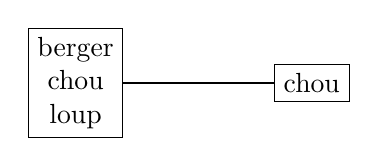
\begin{tikzpicture}[every text node part/.style={align=center}]
\node[draw] (A)at(0,0) {berger \\ chou \\ loup};
\node[draw] (B)at(3,0) {chou};

\draw[-,>=latex] (A) -- (B);
\end{tikzpicture}
\captionof{figure}{Exemple de transition}
\label{transition}
\end{center}
\begin{activite}
Construire le graphe des états de la rive de départ.
\end{activite}
\subsection{Solution}
\begin{activite}
\begin{enumerate}
\item À partir du graphe, trouver une solution pour que le berger transporte tout le monde sur l'autre rive.
\item Existe-t-il un plus court chemin?
\end{enumerate}
\end{activite}
\section{Résolution informatique}
\subsection{Résoudre le problème}
\begin{activite}
En utilisant la classe \emph{Graphe} construite en cours, retrouver et afficher le nombre de transition minimal que doit effectuer le berger.
\end{activite}
\subsection{Visualiser la solution}
La bibliothèque \emph{networkx} permet de construire mais également visualiser des graphes. 
\begin{activite}
En s'aidant de la documentation en ligne, utiliser la bibliothèque \emph{networkx} pour réaliser le graphe résolvant la devinette.
\end{activite}
\end{Form}
\end{document}